                  
% !Mode:: "TeX:UTF-8"

Neste capítulo serão apresentadas as funcionalidades disponíveis aos operadores após a instalação do sistema e cadastro dos mesmos.
A parte do operador é destinada à listagem dos certificados emitidos para sua organização. É possível ver as estatísticas destes certificados e mapear os atributos dos mesmos corretamente.

\section{Certificados}

No menu \textit{Certificados} é possível listar todos os certificados emitidos até o momento para a organização na qual o operador está afiliado, estejam eles ativos ou revogados. Acesse o menu \textit{Certificados $>$ Listar}. Aparecerá uma tela como mostra a figura \ref{fig:listarcertop}. Nesta página é possível ver a data em que foi emitido e a data em que irá expirar cada certificado e o estado em que se encontra (Ativo ou revogado).
É possível realizar as seguintes ações:

\begin{itemize}

	\item \textbf{Download do certificado(}\begin{wrapfigure} 
\includegraphics[height=10]{images/iconedownload} \end{wrapfigure} \textbf{):} Ao clicar nesse ícone você faz o download do certificado selecionado.
	\item \textbf{Revogar certificado(}\begin{wrapfigure} 
\includegraphics[height=10]{images/iconedelete2} \end{wrapfigure} \textbf{):} Quando um certificado estiver ativo, este ícone irá aparecer na linha do respectivo certificado para que este possa ser revogado individualmente. Se houver necessidade de revogar mais certificados, é possível selecioná-los e revogalos de uma só vez através do ícone de revogação no canto inferior direito da imagem. 
	
\end{itemize}

\begin{figure}[ht]
     \centering
     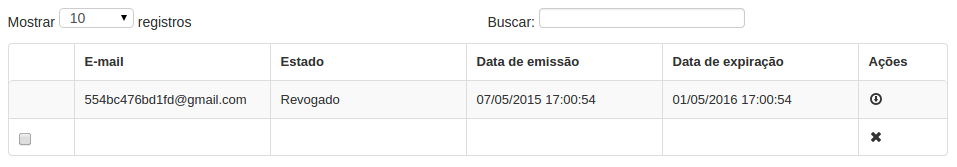
\includegraphics[scale=0.5]{images/listarcertop.png}
     \caption{Listagem de certificados}
     \label{fig:listarcertop}
\end{figure}

\section{Estatísticas}

Esta parte do sistema destina-se à mostrar as estatísticas dos certificados emitidos. É possível verificar quantos certificados já foram emitidos e quantos ainda estão ativos.

\subsection{Total}

Acesse o menu \textit{Estatísticas $>$ Total}. Aparecerá uma tela como mostra a figura \ref{fig:estotalop}. É possível ver quantos certificados já foram emitidos no total, bem como quantos ainda estão ativos, quantos já foram revogados e quantos estão expirados. Lembrando que, diferentemente do perfil de administrador, que pode ver as estatísticas por organização, neste perfil o operador verá apenas a estatística que diz respeito à organização na qual está afiliado.

\begin{figure}[ht]
     \centering
     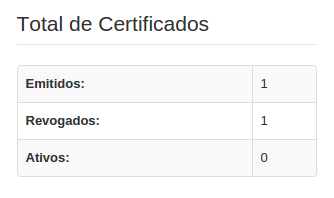
\includegraphics[scale=0.6]{images/estatisticaop.png}
     \caption{Estatísticas total}
     \label{fig:estotalop}
\end{figure}

\subsection{Procurar por tempo}

Acesse o menu \textit{Estatísticas $>$ Procurar por tempo}. Aparecerá uma tela como mostra a figura \ref{fig:estempo}.

\begin{figure}[ht]
     \centering
     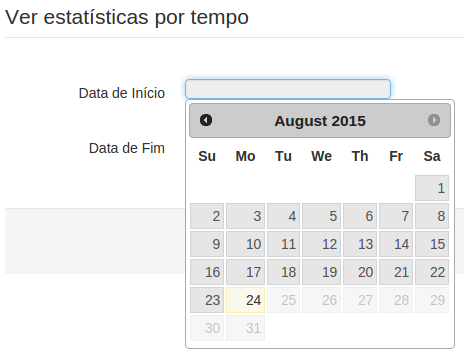
\includegraphics[scale=0.5]{images/estatisticatempo.png}
     \caption{Estatísticas por tempo}
     \label{fig:estempo}
\end{figure}

Para ver a estatística dos certificados emitidos em um período específico de tempo, escolha a data de início e fim e clique no botão \emph{Ver Estatísticas}.

\section{Atributos}

Através do menu \textit{Atributos $>$ Mapeador de atributos} o operador pode configurar os dados que vêm da federação e que vão pertencer ao certificado, como mostra a figura \ref{fig:atmapop}.

\begin{figure}[ht]
     \centering
     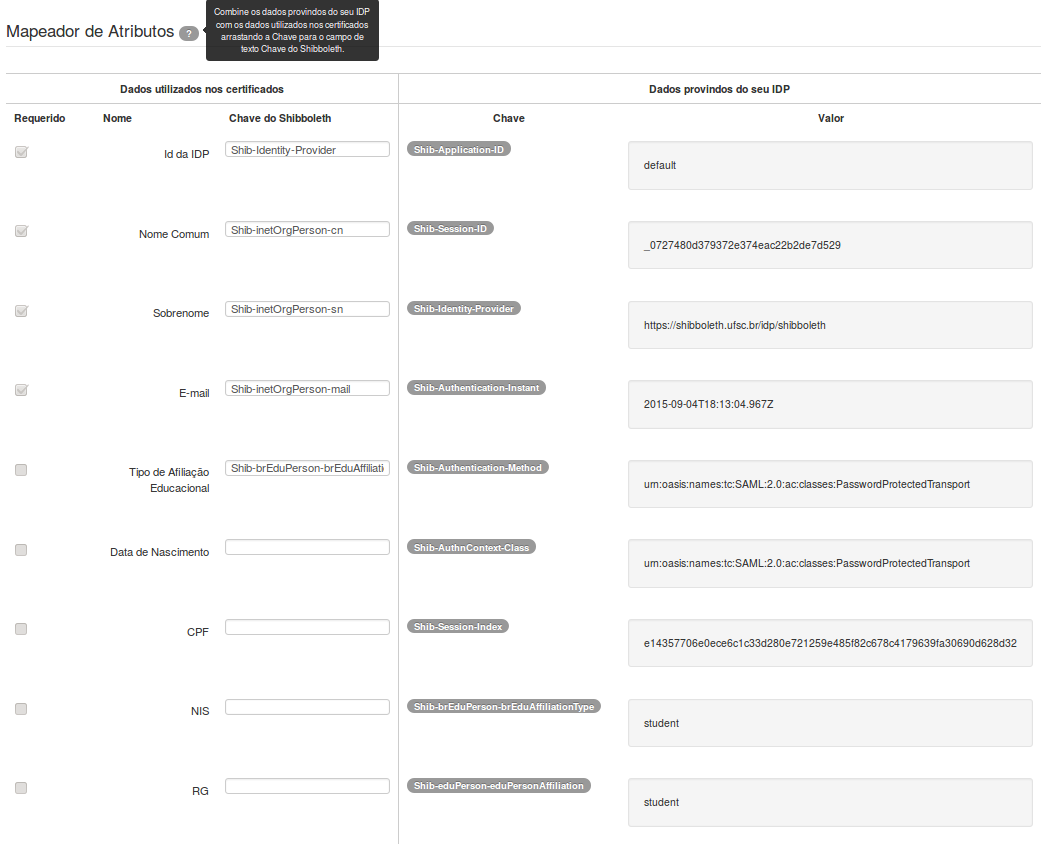
\includegraphics[scale=0.4]{images/oper_attributesmapper.png}
     \caption{Mapeador de atributos}
     \label{fig:atmapop}
\end{figure}

Quando o operador acessar esta tela, os atributos que são necessários configurar já vão vir marcados, pois é o administrador que determina quais atributos vão aparecer no certificado. A tarefa do operador é verificar cada dado que vem da federação e colocá-lo no campo adequado. Por exemplo: Se o CPF for um atributo obrigatório, selecione o CPF na coluna direita, onde estão os dados da federação, e arraste-o para o respectivo campo de CPF na coluna esquerda, onde estão os dados do certificado. Qualquer dúvida que o operador tenha, basta passar o mouse por cima do ponto de interrogação no lado superior esquerdo da tela e encontrará explicação da tarefa. 

\section{Alterar dados do usuário e Sair}

O operador poder alterar seus dados pessoais e sair do sistema a qualquer momento, basta clicar na engrenagem localizada ao lado superior direito da tela. Duas operações aparecerão: \textit{Alterar dados do usuário} e \textit{Sair}. Ao clicar em \textit{Alterar dados do usuário}, aparecerá uma tela com os campos de dados pessoais, como mostra a figura \ref{fig:alterarop}. Altere o que desejar, lembrando que não é possível alterar sua organização. Insira a sua senha e clique no botão \emph{Submeter}. Ao clicar em \textit{Sair}, o usuário sai do sistema.

\begin{figure}[ht]
    \centering
     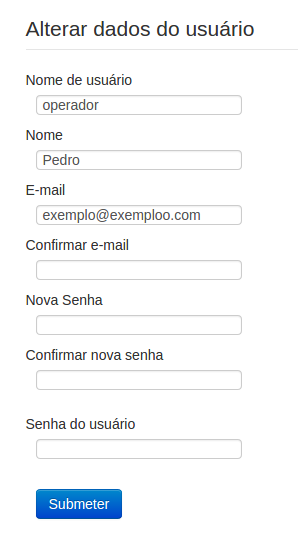
\includegraphics[scale=0.7]{images/alterardadosop.png}
     \caption{Alterar dados do usuário}
     \label{fig:alterarop}
\end{figure}